% !TEX root = ../main.tex

\section{Theory}

% \begin{itemize}
%     \item What is deconvolution and different formulations presented as a review.
%     \item Analysis vs synthesis
%     \begin{itemize}
%         \item TA paper but without the spatial regularization
%         \item PFM paper
%         \item In Gitelman it's an \(\mathbf{H}\) multiplied by a Fourier term.
%     \end{itemize}
%     \item Spikes and block models
% \end{itemize}

\todo[inline]{I think we need a short paragraph here introducing: 1) our notations (vectors, matrices, discrete, continuous); 2) basic math definitions, in particular for norms.}
\subsection{Notations and definitions}

Let us begin by introducing some key notations and definitions. Matrices are denoted by boldface capital letters, e.g., $\mathbf{H}$, vectors are denoted by boldface lowercase letters, e.g., $\mathbf{y}$, and scalars are denoted by lowercase letters, e.g., $k$. Continuous functions are denoted by brackets, e.g., $h(t)$, while discrete functions are denoted by square brackets, e.g., $x[k]$.

The euclidean norm of a matrix $\mathbf{Y}$ is denoted by $\| \mathbf{Y} \|_2$, and the quadratic distance between two matrices $\mathbf{Y}$ and $\mathbf{X}$ is denoted by $\| \mathbf{Y} - \mathbf{X} \|_2^2$. Likewise, the $\ell_1$-norm of a matrix $\mathbf{S}$ is denoted by $\| \mathbf{S} \|_1$.

\subsection{Conventional general linear model analysis}

Conventional general linear model (GLM) analysis puts forward a number of regressors incorporating knowledge about the paradigm or behavior. For instance, the timing of epochs for a certain condition can be modeled as an indicator function $p(t)$, convolved with the HRF $h(t)$, and sampled at TR resolution (\citealt{friston1994analysis, friston1998event, boynton1996linear, cohen1997parametric}):\todo{Rather some Friston paper(s) here}
$$
   p(t) \rightarrow p*h(t) \rightarrow x[k] = p*h(k\cdot\text{TR}).
$$
The vector $\mathbf{x}=[x[k]]_{k=1,\ldots,N}$ then constitutes the hypothetical response, and several of them can be stacked as the columns of the design matrix $\mathbf{X}=[\mathbf{x}_1 \ldots \mathbf{x}_L]$, leading to the celebrated GLM: 
\begin{equation}
    \label{eq:glm}
    \mathbf{y} = \mathbf{X} \boldsymbol\beta + \mathbf{e},
\end{equation}
where the empirical timecourse $\mathbf{y}$ is explained by a linear combination of the regressors in $\mathbf{X}$ weighted by the parameter weights in $\boldsymbol\beta$ and corrupted by additive noise $\mathbf{e}$. Under independent and identically distributed Gaussian assumptions of the latter, the maximum likelihood estimate of the parameter weights reverts to the ordinary least-squares estimator; i.e., minimizing the residual sum of squares between the fitted model and measurements. The number of regressors $L$ is typically much less than the number of measurements $N$, and thus the regression problem is over-determined and does no require additional constraints or assumptions.

In the deconvolution approach, no prior knowledge is taken into account, and the purpose is to estimate the deconvolved activity-inducing signal $\mathbf{s}$ from the measurements $\mathbf{y}$, which can be formulated as the signal model
\begin{equation}
    \label{eq:deconvolution}
    \mathbf{y} = \mathbf{Hs} + \mathbf{e},
\end{equation}
where $\mathbf{H}$ is an $N\times N$ Toeplitz matrix that represents the discrete convolution with the HRF, and $\mathbf{s}$ a length-$N$ vector with the unknown activity-inducing signal. Despite the apparent similarity with the GLM equation, there are two important differences. First, the multiplication with the design matrix of the GLM is an expansion as a weighted linear combination of its columns, while the multiplication with the HRF matrix represents a convolution with its shifted rows. Second, determining $\mathbf{s}$ is an ill-posed problem given the nature of the HRF; e.g., as can be seen intuitively, the rows of $\mathbf{H}$ are highly correlated due to large overlap between shifted HRFs (see Figure~\ref{fig:hrf_diff}B), thus introducing ambiguity and instability in the estimates of $\mathbf{s}$. Therefore, additional assumptions under the form of regularization are needed. 

%%%%%%%%%%%%%%%%%%%%%%%%%%%%%%%%%%%%%%%%%%%%%%%%%%%%%%%%%%%%%%%%%%%%%%%%
% Paradigm Free Mapping
%%%%%%%%%%%%%%%%%%%%%%%%%%%%%%%%%%%%%%%%%%%%%%%%%%%%%%%%%%%%%%%%%%%%%%%%

\subsection{Paradigm-free mapping}
The first approach for deconvolution is based on the forward model formulation of Eq.~(\ref{eq:deconvolution}); i.e., the to-be-recovered activity-inducing signal $\hat{\mathbf{s}}$ is convolved by the HRF and compared against the measured timecourse in the least-squares sense: 
\begin{equation}
    \label{eq:pfm}
    \hat{\mathbf{s}} = \arg \min_{\mathbf{s}} \frac{1}{2} \| \mathbf{y} - \mathbf{Hs} \|_2^2 + \Omega(\mathbf{s}).
\end{equation}
The first term quantifies data fitness, which can be justified as the log-likelihood term derived from Gaussian noise assumptions, while the second term \(\Omega(\mathbf{s})\) brings in regularization and be interpreted as a prior on the activity-inducing signal. In classical Wiener deconvolution, the (squared) $\ell_2$-norm of $\mathbf{s}$ is imposed (i.e., $\Omega(\mathbf{s})=\lambda \left\| \mathbf{s}\right\|_2^2$), which introduces a trade-off, controlled by the regularization parameter $\lambda$, between data fit and ``energy'' of the solution. In paradigm-free mapping (PFM), the formulation of Eq.~(\ref{eq:pfm}) was considered equivalently as fitting the measurements using the atoms of a dictionary (columns of $\mathbf{H}$) with corresponding weights (entries of $\mathbf{s}$) (\citealt{gaudes2011DetectionCharacterizationSingletrial,caballerogaudes2013ParadigmFreeMapping,urunuela2020StabilityBasedSparseParadigm}). 
In addition, sparsity-pursuing regularization was introduced on $\mathbf{s}$, which in a strict way reverts to choosing \(\Omega(\mathbf{s})=\lambda \| \mathbf{s} \|_0\) and solving the optimization problem (\citealt{bruckstein2009SparseSolutionsSystems}). However, due to the convolution model\todo{Even without would be the case, right?} defined in~\eqref{eq:pfm}, finding the optimal solution to the problem demands an exhaustive search across all possible combinations of the columns of \(\mathbf{H}\). Hence, a  pragmatic solution is to solve the convex-relaxed optimization problem for the \(l_1\)-norm, commonly known as the LASSO (\citealt{tibshirani1996RegressionShrinkageSelection}): 
\begin{equation}
    \label{eq:pfm_spike}
    \hat{\mathbf{s}} = \arg \min_{\mathbf{s}} \frac{1}{2} \| \mathbf{y} - \mathbf{Hs} \|_2^2 + \lambda \| \mathbf{s} \|_1,
\end{equation}
which provides fast convergence to a global solution. From the neuronal perspective, imposing sparsity on the activity-inducing signal expresses that activity, at the fMRI timescale of seconds, is supposed to be short and typically can be explained by a small number of large entries. Further on, we refer to this assumption as the spike model. 

%%%%%%%%%%%%%%%%%%%%%%%%%%%%%%%%%%%%%%%%%%%%%%%%%%%%%%%%%%%%%%%%%%%%%%%%
% Total Activation
%%%%%%%%%%%%%%%%%%%%%%%%%%%%%%%%%%%%%%%%%%%%%%%%%%%%%%%%%%%%%%%%%%%%%%%%

\subsection{Total activation}
Alternatively,  deconvolution can be formulated as a denoising problem where the signal to be recovered is directly fitting the measurements and at the same time satisfying some suitable regularization, which leads to
\begin{equation}
    \hat{\mathbf{x}} = \arg \min_{\mathbf{x}} \frac{1}{2} \| \mathbf{y} - \mathbf{x} \|_2^2 + \Omega(\mathbf{x}).
\end{equation}
Well-known regularized regression techniques such as ridge regression (i.e., $\Omega(\mathbf{x})=\lambda\|\mathbf{x}\|_2^2$) and elastic net (i.e., $\Omega(\mathbf{x})=\lambda_1\|\mathbf{x}\|_2^2 + \lambda_2\|\mathbf{x}\|_1$) fall under this category [REF]. One other powerful regularizer is total variation (TV), which is the $\ell_1$-norm of the derivative, $\Omega(\mathbf{x})=\lambda \|\mathbf{Dx}\|_1$, and favors recovery of piecewise-constant signals [REF]. The approach of generalized TV introduces an additional differential operator $\mathbf{D_H}$ in the regularizer that can be tailored as the inverse operator of a linear system~(\citealt{karahanoglu2011SignalProcessingApproacha}), that is, $\Omega(\mathbf{x})=\lambda \|\mathbf{D D_H x}\|_1$. In the context of hemodynamic deconvolution, total activation is proposed for which the discrete operator $\mathbf{D_H}$ is derived from the inverse of the continuous-domain linearized balloon-windkessel model. Exchanging the poles and zeros of the latter's linear-system characterization leads to a differential operator of the form 
\begin{equation}
    D_H\ = \prod_{i=1}^{M_1} (D-\alpha_i I) (\prod_{j=1}^{M_2} (D - \gamma_j I))^{-1},
\end{equation}
where \(D\) is the derivative operator, \(\alpha_i\) the zeros, and \(\gamma_j\) the poles. The interested reader is referred to (\citealt{karahanoglu2013TotalActivationfMRI}) for a detailed description. 

Therefore, the solution of the total-activation problem 
\begin{equation}
    \hat{\mathbf{x}} = \arg \min_{\mathbf{x}} \frac{1}{2} \| \mathbf{y} - \mathbf{x} \|_2^2 + \lambda \| \mathbf{D D_H x} \|_1
\end{equation}
will render the activity-related signal $\mathbf{x}$ for which the activity-inducing signal $\mathbf{s}=\mathbf{D_H x}$ and so-called innovation signal $\mathbf{u}=\mathbf{Ds}$ will also be available, as they are required for the regularization. We refer to the assumption for the activity-inducing signal as the block model.

\subsection{Unifying both perspectives}
\todo[inline]{I would go for a schematic block-flowchart that goes between activity-related/inducing/innovation signals with between each step the two operators; i.e., $\mathbf{H}$ and $\mathbf{D_H}$ for the first, $\mathbf{L}$ and $\mathbf{D}$ for the second.}

PFM and TA are based on the synthesis- and analysis-based formulation of the deconvolution problem, respectively. In the first case, the recovered deconvolved signal is synthesized to be matched to the measurements, while in the second case, the recovered signal is directly matched to the measurements but needs to satisfy its analysis in terms of deconvolution. This also corresponds to using the forward or backward model of the hemodynamic system, respectively. Both approaches are equivalent\footnote{Without dwelling into technicalities, this equivalence is correct up to the constant, which is in the null space of the derivative operator.} [REF Elad\todo{Would be nice to check a bit closer, this is what I concluded.}]. First, TA can be made equivalent to PFM by removing the derivative operator of TA's regularizer. It can then be readily verified that replacing in that case $\mathbf{x}=\mathbf{Hs}$ leads to identical equations and thus both assume a spike model. Second, PFM can also be made equivalent to TA, by considering the modified forward model
$$
\mathbf{y} = \mathbf{H L u} + \mathbf{e},
$$
where the activity-inducing signal $\mathbf{s}$ is rewritten in terms of the innovation signal $\mathbf{u}$; i.e., the derivative $\mathbf{Ds}=\mathbf{u}$ of $\mathbf{s}$ (\citealt{cherkaoui2019SparsitybasedBlindDeconvolution,urunuela2020StabilityBasedSparseParadigm}). This way, PFM will solve for the innovation signal $\mathbf{u}$: 
\begin{equation}
    \label{eq:pfm_block}
    \hat{\mathbf{u}} = \arg \min_{\mathbf{u}} \frac{1}{2} \| \mathbf{y} - \mathbf{HLu} \|_2^2 + \lambda \| \mathbf{u} \|_1,
\end{equation}
and becomes equivalent to TA by replacing $\mathbf{u}=\mathbf{D D_H x}$, and thus adopting the block model.

\begin{figure}[H]
    \begin{center}
        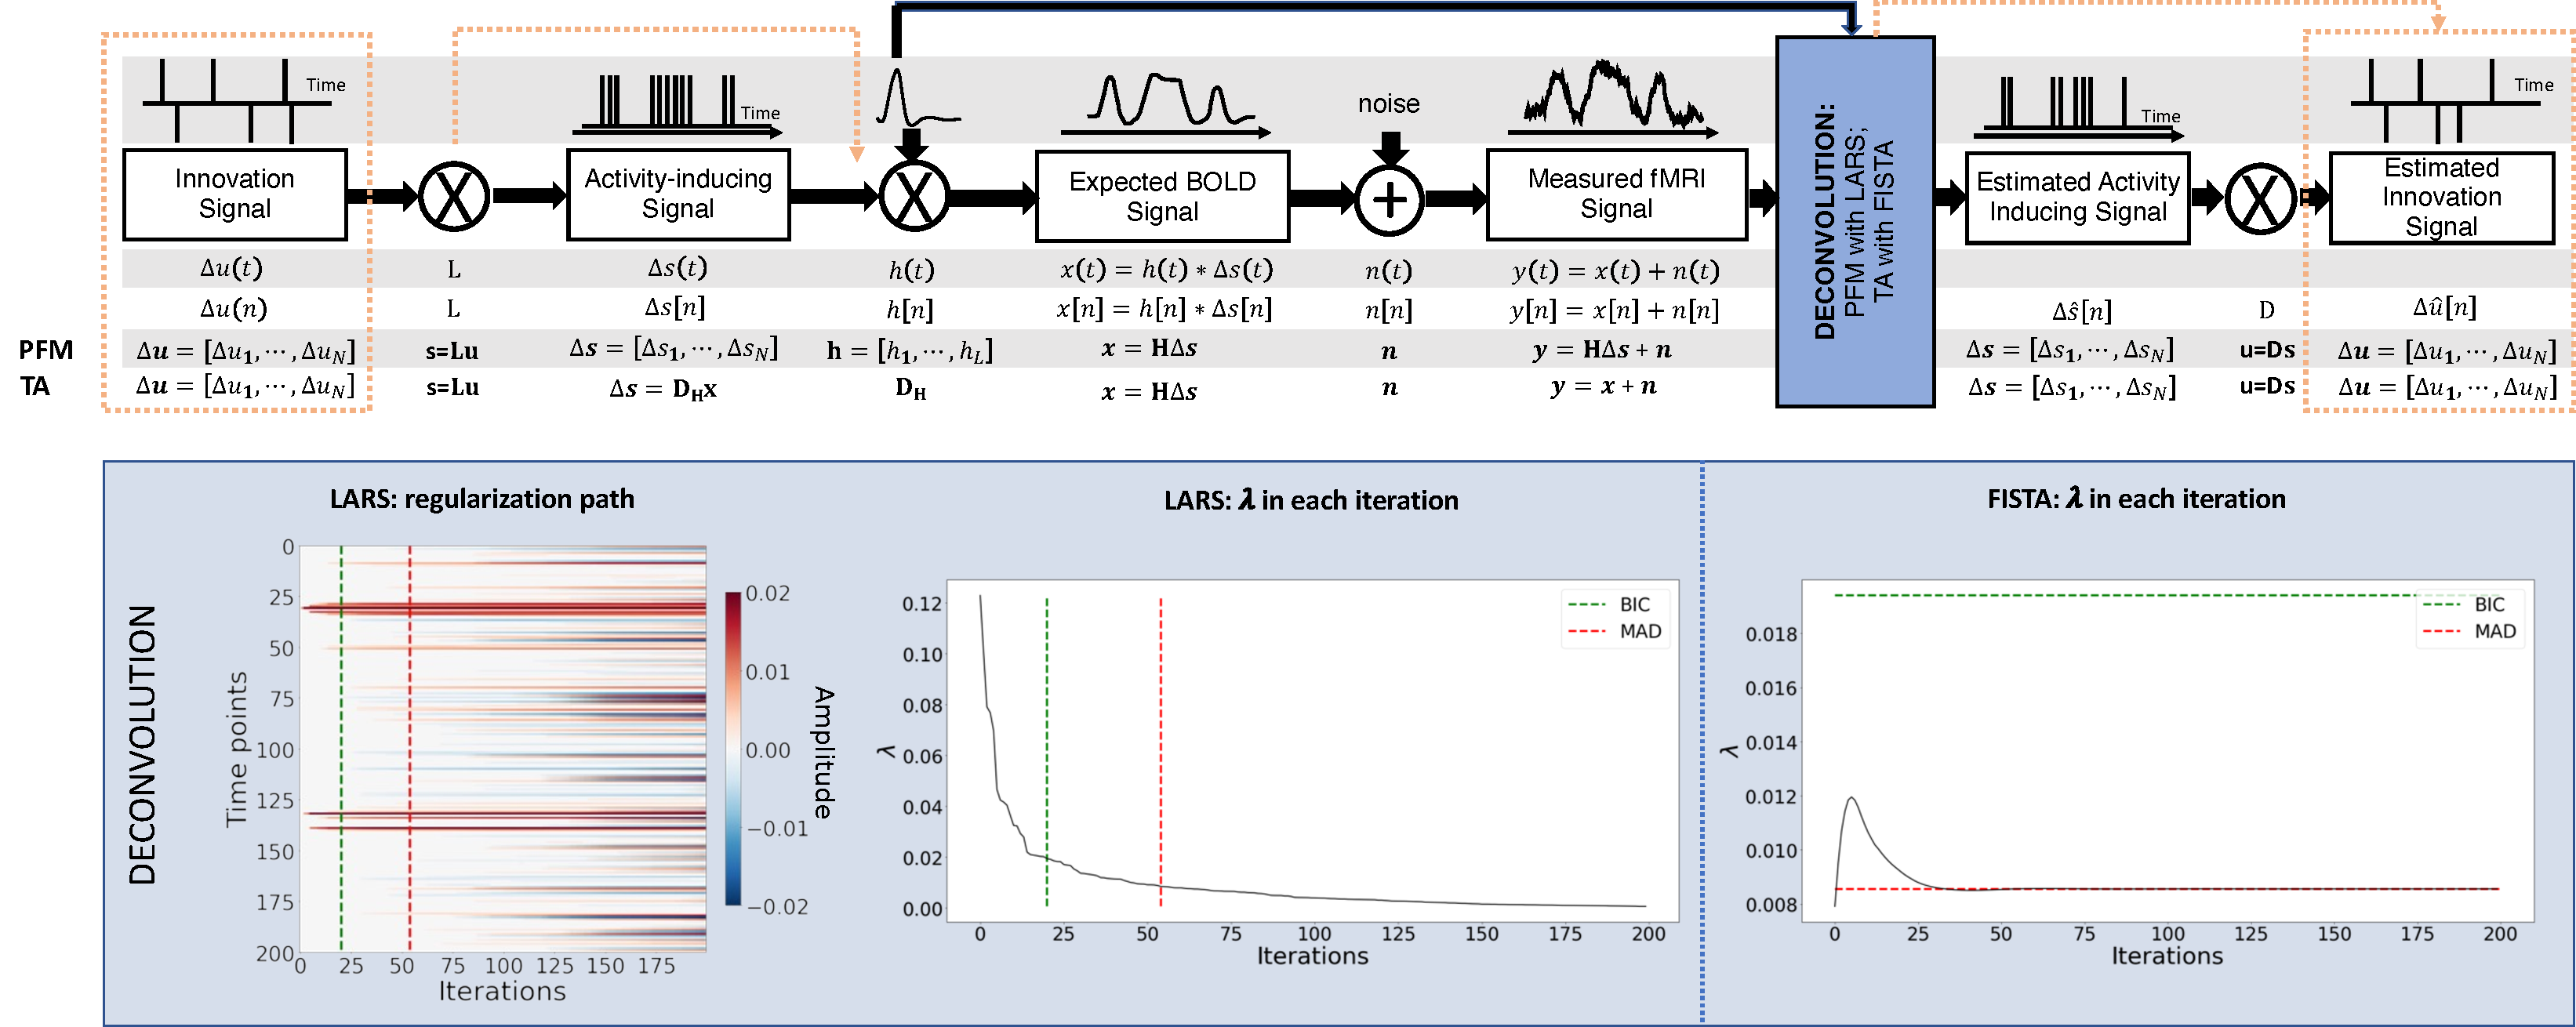
\includegraphics[width=\columnwidth]{figures/flowchart.pdf}
    \end{center}
    \caption{Flowchart detailing the different steps of the fMRI signal and the deconvolution methods described. The orange arrows indicate the flow to estimate the innovation signals. The blue box depicts the two algorithms used in this paper to solve the PFM and TA deconvolution problems.}
\label{fig:flowchart}
\end{figure}

\subsection{Algorithms and parameter selection}
\label{sec:regparam}
\todo[inline]{I think we need a subsection here that gives a brief overview of the different computational approaches to solve PFM and TA. In particular, I think that for the first Figure mentioned above, we could have a second panel (b) in which we put a flowchart of LARS and FGP to illustrate the main idea. -- maybe the parameter selection can be actually merged into this subsection as it will depend on the algorithm.}

Despite their algebraic equivalence, both techniques are solved with different techniques. Here, we evaluate PFM and TA solved using least angle regression (LARS) (\citealt{efron2004LeastAngleRegression}) and fast iterative shrinkage-thresholding algorithm (FISTA) (\citealt{beck2009FastIterativeShrinkagethresholding}), respectively.

In both cases, the correct selection of the regularization parameter $\lambda$ is a critical decision for the accurate performance of deconvolution methods. Even though many techniques have been proposed in the literature, the optimal strategy that selects $\lambda$ is yet to be found. For instance, LARS provide all the possible solutions to the optimization problem and their corresponding value of $\lambda$, i.e., the regularization path, but do not provide the optimal solution. Therefore, strategies that exploit the regularization path can provide a selection of $\lambda$ that is close to the optimal. In the case of PFM, the optimal result is given by the Bayesian Information Criterion (BIC) (\citealt{schwarz1978EstimatingDimensionModel}), i.e., the regularization path solution with the minimum BIC is considered an appropriate solution. In the case of TA, the regularization parameter $\lambda$ is updated on every iteration $n$, so that the residuals converge to a previously estimated noise level of the data fit $\tilde{\sigma}$. The pre-estimated noise level is calculated from the median absolute deviation (MAD) of fine-scale wavelet coefficients (Daubechies, order 3) (\citealt{karahanoglu2013TotalActivationfMRI}):
\begin{equation}
    \lambda^{n+1} = \frac{N \tilde{\sigma}}{\frac{1}{2} \| \mathbf{y} - \mathbf{x}^n \|_F^2} \lambda^n,
\label{eq:std}
\end{equation}
where $x^n$ is the $n^{th}$ iteration estimate, $\lambda^n$ and $\lambda^{n+1}$ are the $n^{th}$ and $n+1^{th}$ iteration values for the regularization parameter $\lambda$, and $N$ is the number of points in the time-course.

% two techniques, i.e., the regularized least-squares problem with temporal regularization, which corresponds to the generalized total-variation operator in Total Activation. Therefore, we do not study the impact of spatial constraints, as we assume that spatial regularization terms should perform identically on both methods.
